%----------------------------------------------------------------------------
\chapter{Implementáció}
%----------------------------------------------------------------------------

\section{Tanítóadatok előkészítése}

A letöltött tanítóadatokat NeMo által értelemzhető formátumúra kellett hozni. Ez magába foglalta a fájlok konvártálását .wav formátumba. Az egyes tanítóadatok más-más formátumban (.opus, .flac, .mp3) voltak eredetileg, illetve eltérő fájstruktúrákba voltak szervezve.

A konvertáláshoz a fentiek miatt a python os könyvtárának walk metódusát használtam mellyel egy mappát rekúrzívan be lehet járni. A konvertáláshoz az ffmpeg szoftvert használtam, mivel segítségével több formátum is könnyedén konvertálható .wav formátumba.

A fájlok átalakításán kívül szükséges volt az adatok .json fájljainak elkészítése, mely megmondja, hogy melyik hangfájl hol található, milyen hosszú és mi hangzik el rajta. A NeMo-nak ezután csupán az egyes manifest-eket, .json fájlokat, kellett megadni, azzal a kiegészítéssel, hogy melyiket kívánjuk tanító vagy teszt adathalamznak használni, és a további előfeldolgozási lépéseket már autómatikusan elvégezte. Természetesen több információ tárolását is támogatja a NeMo, de ezek az adatok elengedhetetlenek.

\section{Modellek kimentése és betöltése}

A tanított modelleket el kell menteni későbbi használat végett. Két módszert is alkalmaztam. Az egyik a logoláshoz hasonlóan callback-et használ, mindig a legoptimálisabb eredményt elért epochot menti ki .ckpt fomrátumban, míg az utóbbi módszer a tanítás végén menti ki a modellt .nemo formátumban.

A mentésre a későbbi felhasználás meleltt azért is van szükség, mert a hosszú tanításokat, melyek akár 48 órán át is tarthatnak, szükséges lehet megszakítani. A megszakítás után fontos úgy betölteni a modellt, hogy az továbbtanítható legyen. A NeMo külön kezeli a modellt és a tanítást végző trainert, melykbe külön külön szükséges betölteni a folytatni kívánt checkpoint-ot.

\section{Kalibráció angol nyelv segítségével}

Első lépésként egy kisebb adatbázison, az AN4-en teszteltem a NeMo keretrendszert, a Google Colab segítségével. Az alap paraméterekkel és konfigurációval az elért eredmények elmaradtak a referencia eredményekéhez képest. Az AN4-es tanítás során QuartzNet 5x1-es architektúrájával dolgoztam a kevés mennyiségű adat végett.

A pontosság növelése érdekében az egy gyakran használt módszer az epoch szám növelése. Egy epoch reprezentálja az összes tanítóadaton való kiértékelést és a súlyok javítását a hiba tükrében. Magas epoch szám jobb eredményeket produkál, de vigyázni kell, mert túlzott epoch szám esetében megjelenhet az úgy nevezett túltanítás jelenség. Ez annyit tesz, hogy a túlzottan is megtanulja a modell a tanítóadatokat, azokra nagyon jó eredményt ad, míg általánosan egyre rosszabbul teljesít.

Egy másik fontos paraméter aminek a módosításával növelni lehet az elért pontosságot a learning rate. A learning rate felel a hiba nyomán felmerült tanítás, azaz súlyok korrekciójának mértékéért. Túl nagy lépések, javítások, esetén a loss értéke, amit csökkenteni szeretnénk, túl nagy ugrásokat végez, akár a rossz irányba. Túl alacsony érték esetén lassan éri el a loss a minimum pontját, legyen az globális vagy lokális. Szintén nem kívánt eredmény az alacsony learning rate esetén, hogy a loss értéke ideje korán beragad egy lokális minumum értékben, ami egy nagyobb lépéssel áthidalható lenne.

% gradient descent valami? képpel akár

A fentiek tükrében növeltem az epoch számot és a learning rate-et, 200-ra és 0.02-re. Sikerült egy optimálisabb eredményt elérjek, így a felhasznált paraméterekkel tovább tudtam indulni egy nagyobb adatbázison való tesztelésre.

\begin{figure}[!ht]
\centering
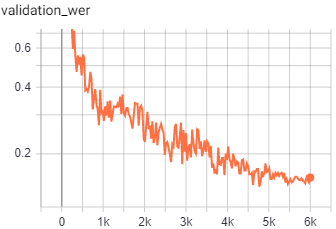
\includegraphics[width=100mm, keepaspectratio]{figures/an4_wer.png}
\caption{AN4 adatbázis validációs adathalmazán elért eredmények.}
\label{fig:TeXstudio}
\end{figure}

Arról, hogy a beállításaim tényleg megfelelőek a LibriSpeech 100 órás adathalmazán bizonyosodtam meg. Azért nem ezzel kezdtem, mert 100 órányi hanganyag tanítása jóval tovább tart, így minél kevesebbszer akartam végigfuttatni a tanítást az optimalizálás érdekében.

A LibriSpeech-hez egy nagyobb méretű architektúrát használtam. A mélyebb hálók jellemzően pontosabb eredményeket képesek elérni a paraméterszám növelése mellett. Összevetettem az eredeti, 5x1-es modellt a nagyobb, 12x1-es QuartzNet modellel és a korábban optimálisnak vélt epoch számmal és egy magasabb learning rate-el. A különbség az 5.2-es ábrán látható.

\begin{figure}[!ht]
\centering
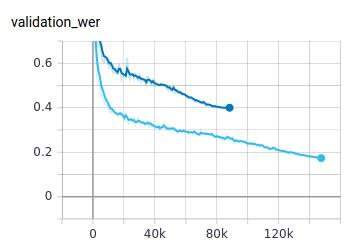
\includegraphics[width=100mm, keepaspectratio]{figures/architecture_comparrison.png}
\caption{LibriSpeech eredmények QuartzNet 5x1 (sötétkék) és 12x1 (világoskék) architektúrákon.}
\label{fig:TeXstudio}
\end{figure}

\section{Orosz nyelvű hálók}

\subsection{Szükséges módosítások}

\subsection{NeMo config fájl}

\subsection{Transfer learning}